\documentclass[1p]{elsarticle_modified}
%\bibliographystyle{elsarticle-num}

%\usepackage[colorlinks]{hyperref}
%\usepackage{abbrmath_seonhwa} %\Abb, \Ascr, \Acal ,\Abf, \Afrak
\usepackage{amsfonts}
\usepackage{amssymb}
\usepackage{amsmath}
\usepackage{amsthm}
\usepackage{scalefnt}
\usepackage{amsbsy}
\usepackage{kotex}
\usepackage{caption}
\usepackage{subfig}
\usepackage{color}
\usepackage{graphicx}
\usepackage{xcolor} %% white, black, red, green, blue, cyan, magenta, yellow
\usepackage{float}
\usepackage{setspace}
\usepackage{hyperref}

\usepackage{tikz}
\usetikzlibrary{arrows}

\usepackage{multirow}
\usepackage{array} % fixed length table
\usepackage{hhline}

%%%%%%%%%%%%%%%%%%%%%
\makeatletter
\renewcommand*\env@matrix[1][\arraystretch]{%
	\edef\arraystretch{#1}%
	\hskip -\arraycolsep
	\let\@ifnextchar\new@ifnextchar
	\array{*\c@MaxMatrixCols c}}
\makeatother %https://tex.stackexchange.com/questions/14071/how-can-i-increase-the-line-spacing-in-a-matrix
%%%%%%%%%%%%%%%

\usepackage[normalem]{ulem}

\newcommand{\msout}[1]{\ifmmode\text{\sout{\ensuremath{#1}}}\else\sout{#1}\fi}
%SOURCE: \msout is \stkout macro in https://tex.stackexchange.com/questions/20609/strikeout-in-math-mode

\newcommand{\cancel}[1]{
	\ifmmode
	{\color{red}\msout{#1}}
	\else
	{\color{red}\sout{#1}}
	\fi
}

\newcommand{\add}[1]{
	{\color{blue}\uwave{#1}}
}

\newcommand{\replace}[2]{
	\ifmmode
	{\color{red}\msout{#1}}{\color{blue}\uwave{#2}}
	\else
	{\color{red}\sout{#1}}{\color{blue}\uwave{#2}}
	\fi
}

\newcommand{\Sol}{\mathcal{S}} %segment
\newcommand{\D}{D} %diagram
\newcommand{\A}{\mathcal{A}} %arc


%%%%%%%%%%%%%%%%%%%%%%%%%%%%%5 test

\def\sl{\operatorname{\textup{SL}}(2,\Cbb)}
\def\psl{\operatorname{\textup{PSL}}(2,\Cbb)}
\def\quan{\mkern 1mu \triangleright \mkern 1mu}

\theoremstyle{definition}
\newtheorem{thm}{Theorem}[section]
\newtheorem{prop}[thm]{Proposition}
\newtheorem{lem}[thm]{Lemma}
\newtheorem{ques}[thm]{Question}
\newtheorem{cor}[thm]{Corollary}
\newtheorem{defn}[thm]{Definition}
\newtheorem{exam}[thm]{Example}
\newtheorem{rmk}[thm]{Remark}
\newtheorem{alg}[thm]{Algorithm}

\newcommand{\I}{\sqrt{-1}}
\begin{document}

%\begin{frontmatter}
%
%\title{Boundary parabolic representations of knots up to 8 crossings}
%
%%% Group authors per affiliation:
%\author{Yunhi Cho} 
%\address{Department of Mathematics, University of Seoul, Seoul, Korea}
%\ead{yhcho@uos.ac.kr}
%
%
%\author{Seonhwa Kim} %\fnref{s_kim}}
%\address{Center for Geometry and Physics, Institute for Basic Science, Pohang, 37673, Korea}
%\ead{ryeona17@ibs.re.kr}
%
%\author{Hyuk Kim}
%\address{Department of Mathematical Sciences, Seoul National University, Seoul 08826, Korea}
%\ead{hyukkim@snu.ac.kr}
%
%\author{Seokbeom Yoon}
%\address{Department of Mathematical Sciences, Seoul National University, Seoul, 08826,  Korea}
%\ead{sbyoon15@snu.ac.kr}
%
%\begin{abstract}
%We find all boundary parabolic representation of knots up to 8 crossings.
%
%\end{abstract}
%\begin{keyword}
%    \MSC[2010] 57M25 
%\end{keyword}
%
%\end{frontmatter}

%\linenumbers
%\tableofcontents
%
\newcommand\colored[1]{\textcolor{white}{\rule[-0.35ex]{0.8em}{1.4ex}}\kern-0.8em\color{red} #1}%
%\newcommand\colored[1]{\textcolor{white}{ #1}\kern-2.17ex	\textcolor{white}{ #1}\kern-1.81ex	\textcolor{white}{ #1}\kern-2.15ex\color{red}#1	}

{\Large $\underline{12a_{0731}~(K12a_{0731})}$}

\setlength{\tabcolsep}{10pt}
\renewcommand{\arraystretch}{1.6}
\vspace{1cm}\begin{tabular}{m{100pt}>{\centering\arraybackslash}m{274pt}}
\multirow{5}{120pt}{
	\centering
	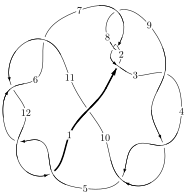
\includegraphics[width=112pt]{../../../GIT/diagram.site/Diagrams/png/1532_12a_0731.png}\\
\ \ \ A knot diagram\footnotemark}&
\allowdisplaybreaks
\textbf{Linearized knot diagam} \\
\cline{2-2}
 &
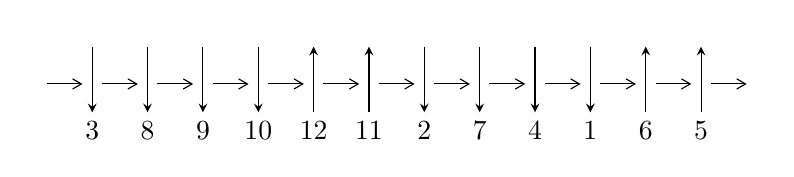
\begin{tikzpicture}[x=20pt, y=17pt]
	% nodes
	\node (C0) at (0, 0) {};
	\node (C1) at (1, 0) {};
	\node (C1U) at (1, +1) {};
	\node (C1D) at (1, -1) {3};

	\node (C2) at (2, 0) {};
	\node (C2U) at (2, +1) {};
	\node (C2D) at (2, -1) {8};

	\node (C3) at (3, 0) {};
	\node (C3U) at (3, +1) {};
	\node (C3D) at (3, -1) {9};

	\node (C4) at (4, 0) {};
	\node (C4U) at (4, +1) {};
	\node (C4D) at (4, -1) {10};

	\node (C5) at (5, 0) {};
	\node (C5U) at (5, +1) {};
	\node (C5D) at (5, -1) {12};

	\node (C6) at (6, 0) {};
	\node (C6U) at (6, +1) {};
	\node (C6D) at (6, -1) {11};

	\node (C7) at (7, 0) {};
	\node (C7U) at (7, +1) {};
	\node (C7D) at (7, -1) {2};

	\node (C8) at (8, 0) {};
	\node (C8U) at (8, +1) {};
	\node (C8D) at (8, -1) {7};

	\node (C9) at (9, 0) {};
	\node (C9U) at (9, +1) {};
	\node (C9D) at (9, -1) {4};

	\node (C10) at (10, 0) {};
	\node (C10U) at (10, +1) {};
	\node (C10D) at (10, -1) {1};

	\node (C11) at (11, 0) {};
	\node (C11U) at (11, +1) {};
	\node (C11D) at (11, -1) {6};

	\node (C12) at (12, 0) {};
	\node (C12U) at (12, +1) {};
	\node (C12D) at (12, -1) {5};
	\node (C13) at (13, 0) {};

	% arrows
	\draw[->,>={angle 60}]
	(C0) edge (C1) (C1) edge (C2) (C2) edge (C3) (C3) edge (C4) (C4) edge (C5) (C5) edge (C6) (C6) edge (C7) (C7) edge (C8) (C8) edge (C9) (C9) edge (C10) (C10) edge (C11) (C11) edge (C12) (C12) edge (C13) ;	\draw[->,>=stealth]
	(C1U) edge (C1D) (C2U) edge (C2D) (C3U) edge (C3D) (C4U) edge (C4D) (C5D) edge (C5U) (C6D) edge (C6U) (C7U) edge (C7D) (C8U) edge (C8D) (C9U) edge (C9D) (C10U) edge (C10D) (C11D) edge (C11U) (C12D) edge (C12U) ;
	\end{tikzpicture} \\
\hhline{~~} \\& 
\textbf{Solving Sequence} \\ \cline{2-2} 
 &
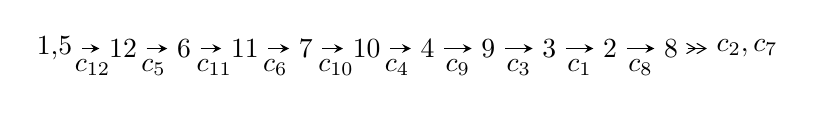
\begin{tikzpicture}[x=22pt, y=7pt]
	% node
	\node (A0) at (-1/8, 0) {1,5};
	\node (A1) at (1, 0) {12};
	\node (A2) at (2, 0) {6};
	\node (A3) at (3, 0) {11};
	\node (A4) at (4, 0) {7};
	\node (A5) at (5, 0) {10};
	\node (A6) at (6, 0) {4};
	\node (A7) at (7, 0) {9};
	\node (A8) at (8, 0) {3};
	\node (A9) at (9, 0) {2};
	\node (A10) at (10, 0) {8};
	\node (C1) at (1/2, -1) {$c_{12}$};
	\node (C2) at (3/2, -1) {$c_{5}$};
	\node (C3) at (5/2, -1) {$c_{11}$};
	\node (C4) at (7/2, -1) {$c_{6}$};
	\node (C5) at (9/2, -1) {$c_{10}$};
	\node (C6) at (11/2, -1) {$c_{4}$};
	\node (C7) at (13/2, -1) {$c_{9}$};
	\node (C8) at (15/2, -1) {$c_{3}$};
	\node (C9) at (17/2, -1) {$c_{1}$};
	\node (C10) at (19/2, -1) {$c_{8}$};
	\node (A11) at (45/4, 0) {$c_{2},c_{7}$};

	% edge
	\draw[->,>=stealth]	
	(A0) edge (A1) (A1) edge (A2) (A2) edge (A3) (A3) edge (A4) (A4) edge (A5) (A5) edge (A6) (A6) edge (A7) (A7) edge (A8) (A8) edge (A9) (A9) edge (A10) ;
	\draw[->>,>={angle 60}]	
	(A10) edge (A11);
\end{tikzpicture} \\ 

\end{tabular} \\

\footnotetext{
The image of knot diagram is generated by the software ``\textbf{Draw programme}" developed by Andrew Bartholomew(\url{http://www.layer8.co.uk/maths/draw/index.htm\#Running-draw}), where we modified some parts for our purpose(\url{https://github.com/CATsTAILs/LinksPainter}).
}\phantom \\ \newline 
\centering \textbf{Ideals for irreducible components\footnotemark of $X_{\text{par}}$} 
 
\begin{align*}
I^u_{1}&=\langle 
u^{52}- u^{51}+\cdots- u^2-1\rangle \\
\\
\end{align*}
\raggedright * 1 irreducible components of $\dim_{\mathbb{C}}=0$, with total 52 representations.\\
\footnotetext{All coefficients of polynomials are rational numbers. But the coefficients are sometimes approximated in decimal forms when there is not enough margin.}
\newpage
\renewcommand{\arraystretch}{1}
\centering \section*{I. $I^u_{1}= \langle u^{52}- u^{51}+\cdots- u^2-1 \rangle$}
\flushleft \textbf{(i) Arc colorings}\\
\begin{tabular}{m{7pt} m{180pt} m{7pt} m{180pt} }
\flushright $a_{1}=$&$\begin{pmatrix}1\\0\end{pmatrix}$ \\
\flushright $a_{5}=$&$\begin{pmatrix}0\\u\end{pmatrix}$ \\
\flushright $a_{12}=$&$\begin{pmatrix}1\\u^2\end{pmatrix}$ \\
\flushright $a_{6}=$&$\begin{pmatrix}u\\u^3+u\end{pmatrix}$ \\
\flushright $a_{11}=$&$\begin{pmatrix}u^2+1\\u^4+2 u^2\end{pmatrix}$ \\
\flushright $a_{7}=$&$\begin{pmatrix}u^3+2 u\\u^5+3 u^3+u\end{pmatrix}$ \\
\flushright $a_{10}=$&$\begin{pmatrix}u^4+3 u^2+1\\u^4+2 u^2\end{pmatrix}$ \\
\flushright $a_{4}=$&$\begin{pmatrix}u^9+6 u^7+11 u^5+6 u^3+u\\u^9+5 u^7+7 u^5+2 u^3+u\end{pmatrix}$ \\
\flushright $a_{9}=$&$\begin{pmatrix}- u^{14}-9 u^{12}-30 u^{10}-45 u^8-30 u^6-8 u^4+2 u^2+1\\- u^{14}-8 u^{12}-23 u^{10}-28 u^8-14 u^6-4 u^4+u^2\end{pmatrix}$ \\
\flushright $a_{3}=$&$\begin{pmatrix}- u^{19}-12 u^{17}+\cdots+11 u^3+2 u\\- u^{19}-11 u^{17}+\cdots+3 u^3+u\end{pmatrix}$ \\
\flushright $a_{2}=$&$\begin{pmatrix}u^{38}+23 u^{36}+\cdots+2 u^2+1\\u^{38}+22 u^{36}+\cdots+6 u^4+u^2\end{pmatrix}$ \\
\flushright $a_{8}=$&$\begin{pmatrix}u^{22}+13 u^{20}+\cdots-15 u^4+1\\u^{24}+14 u^{22}+\cdots-30 u^6-10 u^4\end{pmatrix}$\\&\end{tabular}
\flushleft \textbf{(ii) Obstruction class $= -1$}\\~\\
\flushleft \textbf{(iii) Cusp Shapes $= 4 u^{51}-4 u^{50}+\cdots-12 u-6$}\\~\\
\newpage\renewcommand{\arraystretch}{1}
\flushleft \textbf{(iv) u-Polynomials at the component}\newline \\
\begin{tabular}{m{50pt}|m{274pt}}
Crossings & \hspace{64pt}u-Polynomials at each crossing \\
\hline $$\begin{aligned}c_{1},c_{8}\end{aligned}$$&$\begin{aligned}
&u^{52}+19 u^{51}+\cdots-2 u+1
\end{aligned}$\\
\hline $$\begin{aligned}c_{2},c_{7}\end{aligned}$$&$\begin{aligned}
&u^{52}+u^{51}+\cdots-2 u-1
\end{aligned}$\\
\hline $$\begin{aligned}c_{3},c_{4},c_{9}\end{aligned}$$&$\begin{aligned}
&u^{52}- u^{51}+\cdots-8 u-4
\end{aligned}$\\
\hline $$\begin{aligned}c_{5},c_{6},c_{11}\\c_{12}\end{aligned}$$&$\begin{aligned}
&u^{52}- u^{51}+\cdots- u^2-1
\end{aligned}$\\
\hline $$\begin{aligned}c_{10}\end{aligned}$$&$\begin{aligned}
&u^{52}-17 u^{51}+\cdots-26192 u+2993
\end{aligned}$\\
\hline
\end{tabular}\\~\\
\newpage\renewcommand{\arraystretch}{1}
\flushleft \textbf{(v) Riley Polynomials at the component}\newline \\
\begin{tabular}{m{50pt}|m{274pt}}
Crossings & \hspace{64pt}Riley Polynomials at each crossing \\
\hline $$\begin{aligned}c_{1},c_{8}\end{aligned}$$&$\begin{aligned}
&y^{52}+29 y^{51}+\cdots+18 y+1
\end{aligned}$\\
\hline $$\begin{aligned}c_{2},c_{7}\end{aligned}$$&$\begin{aligned}
&y^{52}-19 y^{51}+\cdots+2 y+1
\end{aligned}$\\
\hline $$\begin{aligned}c_{3},c_{4},c_{9}\end{aligned}$$&$\begin{aligned}
&y^{52}-55 y^{51}+\cdots-184 y+16
\end{aligned}$\\
\hline $$\begin{aligned}c_{5},c_{6},c_{11}\\c_{12}\end{aligned}$$&$\begin{aligned}
&y^{52}+61 y^{51}+\cdots+2 y+1
\end{aligned}$\\
\hline $$\begin{aligned}c_{10}\end{aligned}$$&$\begin{aligned}
&y^{52}-31 y^{51}+\cdots-170476614 y+8958049
\end{aligned}$\\
\hline
\end{tabular}\\~\\
\newpage\flushleft \textbf{(vi) Complex Volumes and Cusp Shapes}
$$\begin{array}{c|c|c}  
\text{Solutions to }I^u_{1}& \I (\text{vol} + \sqrt{-1}CS) & \text{Cusp shape}\\
 \hline 
\begin{aligned}
u &= \phantom{-}0.417129 + 0.833683 I\end{aligned}
 & -6.57030 - 3.29491 I & -10.38217 + 1.00924 I \\ \hline\begin{aligned}
u &= \phantom{-}0.417129 - 0.833683 I\end{aligned}
 & -6.57030 + 3.29491 I & -10.38217 - 1.00924 I \\ \hline\begin{aligned}
u &= \phantom{-}0.447855 + 0.817464 I\end{aligned}
 & -10.54530 + 3.62754 I & -13.7524 - 4.1082 I \\ \hline\begin{aligned}
u &= \phantom{-}0.447855 - 0.817464 I\end{aligned}
 & -10.54530 - 3.62754 I & -13.7524 + 4.1082 I \\ \hline\begin{aligned}
u &= \phantom{-}0.468982 + 0.795969 I\end{aligned}
 & -6.17965 + 10.49310 I & -9.45880 - 8.85692 I \\ \hline\begin{aligned}
u &= \phantom{-}0.468982 - 0.795969 I\end{aligned}
 & -6.17965 - 10.49310 I & -9.45880 + 8.85692 I \\ \hline\begin{aligned}
u &= -0.415985 + 0.814109 I\end{aligned}
 & -4.96278 - 2.01233 I & -8.04647 + 3.92304 I \\ \hline\begin{aligned}
u &= -0.415985 - 0.814109 I\end{aligned}
 & -4.96278 + 2.01233 I & -8.04647 - 3.92304 I \\ \hline\begin{aligned}
u &= -0.456551 + 0.790170 I\end{aligned}
 & -4.67136 - 5.01095 I & -7.40961 + 4.34724 I \\ \hline\begin{aligned}
u &= -0.456551 - 0.790170 I\end{aligned}
 & -4.67136 + 5.01095 I & -7.40961 - 4.34724 I \\ \hline\begin{aligned}
u &= -0.307728 + 0.673902 I\end{aligned}
 & -3.04997 - 2.38050 I & -13.2356 + 6.5396 I \\ \hline\begin{aligned}
u &= -0.307728 - 0.673902 I\end{aligned}
 & -3.04997 + 2.38050 I & -13.2356 - 6.5396 I \\ \hline\begin{aligned}
u &= -0.431177 + 0.595940 I\end{aligned}
 & \phantom{-}1.33174 - 6.67291 I & -4.55025 + 10.19057 I \\ \hline\begin{aligned}
u &= -0.431177 - 0.595940 I\end{aligned}
 & \phantom{-}1.33174 + 6.67291 I & -4.55025 - 10.19057 I \\ \hline\begin{aligned}
u &= -0.075469 + 0.725881 I\end{aligned}
 & -0.97753 + 2.21512 I & -11.08908 - 2.69956 I \\ \hline\begin{aligned}
u &= -0.075469 - 0.725881 I\end{aligned}
 & -0.97753 - 2.21512 I & -11.08908 + 2.69956 I \\ \hline\begin{aligned}
u &= \phantom{-}0.417591 + 0.557999 I\end{aligned}
 & \phantom{-}1.94823 + 1.38800 I & -2.50449 - 4.64036 I \\ \hline\begin{aligned}
u &= \phantom{-}0.417591 - 0.557999 I\end{aligned}
 & \phantom{-}1.94823 - 1.38800 I & -2.50449 + 4.64036 I \\ \hline\begin{aligned}
u &= \phantom{-}0.636854\phantom{ +0.000000I}\end{aligned}
 & -8.09348\phantom{ +0.000000I} & -9.74010\phantom{ +0.000000I} \\ \hline\begin{aligned}
u &= \phantom{-}0.633274 + 0.038957 I\end{aligned}
 & -3.92657 - 6.79204 I & -5.72913 + 4.81858 I \\ \hline\begin{aligned}
u &= \phantom{-}0.633274 - 0.038957 I\end{aligned}
 & -3.92657 + 6.79204 I & -5.72913 - 4.81858 I \\ \hline\begin{aligned}
u &= -0.614460 + 0.031464 I\end{aligned}
 & -2.42291 + 1.41178 I & -3.50849 - 0.14454 I \\ \hline\begin{aligned}
u &= -0.614460 - 0.031464 I\end{aligned}
 & -2.42291 - 1.41178 I & -3.50849 + 0.14454 I \\ \hline\begin{aligned}
u &= \phantom{-}0.241452 + 0.491984 I\end{aligned}
 & -0.158403 + 0.970828 I & -3.16514 - 6.89693 I \\ \hline\begin{aligned}
u &= \phantom{-}0.241452 - 0.491984 I\end{aligned}
 & -0.158403 - 0.970828 I & -3.16514 + 6.89693 I \\ \hline\begin{aligned}
u &= \phantom{-}0.435224 + 0.311244 I\end{aligned}
 & \phantom{-}2.64348 + 1.66592 I & \phantom{-}0.51705 - 3.90838 I \\ \hline\begin{aligned}
u &= \phantom{-}0.435224 - 0.311244 I\end{aligned}
 & \phantom{-}2.64348 - 1.66592 I & \phantom{-}0.51705 + 3.90838 I \\ \hline\begin{aligned}
u &= -0.459005 + 0.259005 I\end{aligned}
 & \phantom{-}2.28374 + 3.52243 I & -0.68639 - 3.07419 I \\ \hline\begin{aligned}
u &= -0.459005 - 0.259005 I\end{aligned}
 & \phantom{-}2.28374 - 3.52243 I & -0.68639 + 3.07419 I \\ \hline\begin{aligned}
u &= \phantom{-}0.01062 + 1.50422 I\end{aligned}
 & -3.13178 + 2.70355 I & \phantom{-0.000000 } 0\\
 \hline 
 \end{array}$$\newpage$$\begin{array}{c|c|c}  
\text{Solutions to }I^u_{1}& \I (\text{vol} + \sqrt{-1}CS) & \text{Cusp shape}\\
 \hline 
\begin{aligned}
u &= \phantom{-}0.01062 - 1.50422 I\end{aligned}
 & -3.13178 - 2.70355 I & \phantom{-0.000000 } 0 \\ \hline\begin{aligned}
u &= \phantom{-}0.09297 + 1.55850 I\end{aligned}
 & -5.18614 + 3.13538 I & \phantom{-0.000000 } 0 \\ \hline\begin{aligned}
u &= \phantom{-}0.09297 - 1.55850 I\end{aligned}
 & -5.18614 - 3.13538 I & \phantom{-0.000000 } 0 \\ \hline\begin{aligned}
u &= -0.10423 + 1.56695 I\end{aligned}
 & -5.96476 - 8.55636 I & \phantom{-0.000000 } 0 \\ \hline\begin{aligned}
u &= -0.10423 - 1.56695 I\end{aligned}
 & -5.96476 + 8.55636 I & \phantom{-0.000000 } 0 \\ \hline\begin{aligned}
u &= \phantom{-}0.04555 + 1.57078 I\end{aligned}
 & -7.31168 + 1.86434 I & \phantom{-0.000000 } 0 \\ \hline\begin{aligned}
u &= \phantom{-}0.04555 - 1.57078 I\end{aligned}
 & -7.31168 - 1.86434 I & \phantom{-0.000000 } 0 \\ \hline\begin{aligned}
u &= -0.07403 + 1.59817 I\end{aligned}
 & -10.82600 - 3.74121 I & \phantom{-0.000000 } 0 \\ \hline\begin{aligned}
u &= -0.07403 - 1.59817 I\end{aligned}
 & -10.82600 + 3.74121 I & \phantom{-0.000000 } 0 \\ \hline\begin{aligned}
u &= -0.02520 + 1.60559 I\end{aligned}
 & -8.95532 + 1.81146 I & \phantom{-0.000000 } 0 \\ \hline\begin{aligned}
u &= -0.02520 - 1.60559 I\end{aligned}
 & -8.95532 - 1.81146 I & \phantom{-0.000000 } 0 \\ \hline\begin{aligned}
u &= -0.386669\phantom{ +0.000000I}\end{aligned}
 & -1.22216\phantom{ +0.000000I} & -7.16550\phantom{ +0.000000I} \\ \hline\begin{aligned}
u &= -0.13033 + 1.63602 I\end{aligned}
 & -12.9782 - 7.2412 I & \phantom{-0.000000 } 0 \\ \hline\begin{aligned}
u &= -0.13033 - 1.63602 I\end{aligned}
 & -12.9782 + 7.2412 I & \phantom{-0.000000 } 0 \\ \hline\begin{aligned}
u &= \phantom{-}0.13423 + 1.63834 I\end{aligned}
 & -14.5123 + 12.7892 I & \phantom{-0.000000 } 0 \\ \hline\begin{aligned}
u &= \phantom{-}0.13423 - 1.63834 I\end{aligned}
 & -14.5123 - 12.7892 I & \phantom{-0.000000 } 0 \\ \hline\begin{aligned}
u &= -0.11630 + 1.64091 I\end{aligned}
 & -13.39160 - 4.03746 I & \phantom{-0.000000 } 0 \\ \hline\begin{aligned}
u &= -0.11630 - 1.64091 I\end{aligned}
 & -13.39160 + 4.03746 I & \phantom{-0.000000 } 0 \\ \hline\begin{aligned}
u &= \phantom{-}0.12590 + 1.64441 I\end{aligned}
 & -18.9946 + 5.8156 I & \phantom{-0.000000 } 0 \\ \hline\begin{aligned}
u &= \phantom{-}0.12590 - 1.64441 I\end{aligned}
 & -18.9946 - 5.8156 I & \phantom{-0.000000 } 0 \\ \hline\begin{aligned}
u &= \phantom{-}0.11458 + 1.64704 I\end{aligned}
 & -15.1010 - 1.2710 I & \phantom{-0.000000 } 0 \\ \hline\begin{aligned}
u &= \phantom{-}0.11458 - 1.64704 I\end{aligned}
 & -15.1010 + 1.2710 I & \phantom{-0.000000 } 0\\
 \hline 
 \end{array}$$\newpage
\newpage\renewcommand{\arraystretch}{1}
\centering \section*{ II. u-Polynomials}
\begin{tabular}{m{50pt}|m{274pt}}
Crossings & \hspace{64pt}u-Polynomials at each crossing \\
\hline $$\begin{aligned}c_{1},c_{8}\end{aligned}$$&$\begin{aligned}
&u^{52}+19 u^{51}+\cdots-2 u+1
\end{aligned}$\\
\hline $$\begin{aligned}c_{2},c_{7}\end{aligned}$$&$\begin{aligned}
&u^{52}+u^{51}+\cdots-2 u-1
\end{aligned}$\\
\hline $$\begin{aligned}c_{3},c_{4},c_{9}\end{aligned}$$&$\begin{aligned}
&u^{52}- u^{51}+\cdots-8 u-4
\end{aligned}$\\
\hline $$\begin{aligned}c_{5},c_{6},c_{11}\\c_{12}\end{aligned}$$&$\begin{aligned}
&u^{52}- u^{51}+\cdots- u^2-1
\end{aligned}$\\
\hline $$\begin{aligned}c_{10}\end{aligned}$$&$\begin{aligned}
&u^{52}-17 u^{51}+\cdots-26192 u+2993
\end{aligned}$\\
\hline
\end{tabular}\newpage\renewcommand{\arraystretch}{1}
\centering \section*{ III. Riley Polynomials}
\begin{tabular}{m{50pt}|m{274pt}}
Crossings & \hspace{64pt}Riley Polynomials at each crossing \\
\hline $$\begin{aligned}c_{1},c_{8}\end{aligned}$$&$\begin{aligned}
&y^{52}+29 y^{51}+\cdots+18 y+1
\end{aligned}$\\
\hline $$\begin{aligned}c_{2},c_{7}\end{aligned}$$&$\begin{aligned}
&y^{52}-19 y^{51}+\cdots+2 y+1
\end{aligned}$\\
\hline $$\begin{aligned}c_{3},c_{4},c_{9}\end{aligned}$$&$\begin{aligned}
&y^{52}-55 y^{51}+\cdots-184 y+16
\end{aligned}$\\
\hline $$\begin{aligned}c_{5},c_{6},c_{11}\\c_{12}\end{aligned}$$&$\begin{aligned}
&y^{52}+61 y^{51}+\cdots+2 y+1
\end{aligned}$\\
\hline $$\begin{aligned}c_{10}\end{aligned}$$&$\begin{aligned}
&y^{52}-31 y^{51}+\cdots-170476614 y+8958049
\end{aligned}$\\
\hline
\end{tabular}
\vskip 2pc
\end{document}